
\section{Navier--Stokes equations with interfaces} 
\label{nse}

We model flows with sharp interfaces defined implicitly by a characteristic function $H(\X,t)$
defined such that fluid 1 corresponds to $H=1$ and fluid 2 to $H=0$. The viscosities $\mu$
and densities $\rho$ are calculated as an average
\be
\mu = \mu_1 H + \mu_2 (1-H)\,, \qquad \rho = \rho_1 H + \rho_2 (1 - H) \,. 
\label{muH}
\nd
There is no phase change so the interface, 
almost always a smooth differentiable surface $S$, advances at the speed of the 
flow, that is $V_S=\U\cdot \N$ where $\U$ is the local fluid velocity 
and $\N$ a unit normal vector perpendicular to the interface. Equivalently 
the interface motion can be expressed in weak form
\be
\dert H + \U \cdot \grad H = 0 \,, 
\label{interfadv}
\nd
which expresses the fact that the singularity of $H$, located on $S$, moves at velocity $V_S=\U\cdot \N$. 
For incompressible flows, which we will consider in what follows, we have
\be
\nabla \cdot \U = 0 \,.
\label{divu}
\nd
The Navier--Stokes equations for incompressible, Newtonian flow with surface tension may 
conveniently be written in operator form
\be
 \dert (\rho \U) = \LLL(\rho,\U) - \grad p \label{nse1}
\nd
where 
$
\LLL =  \LLL_{\rm conv} + \LLL_{\rm diff} +   \LLL_{\rm cap} + \LLL_{\rm ext}
$
so that the operator $\LLL$ is the sum of advective, diffusive, capillary force and
external force terms. The first two terms are 
\be
\LLL_{\rm conv} = -\grad \cdot ( \rho \U  \U )\,, \qquad \LLL_{\rm diff} =  \grad \cdot \DD \,,
\nd
where $\DD$ is a stress tensor whose expression for incompressible flow is
\be
\DD = \mu \left[ \nabla\U + (\nabla\U)^T \right] \,,
\nd
where $\mu$ is computed from $H$ using (\ref{muH}). 
The capillary term is
\be
\LLL_{\rm cap} =  {\sigma \kappa \delta_S \N} \,,  \qquad \kappa = 1/R_1 + 1/R_2 \,,
\nd
where $\sigma$ is the surface tension, $\N$ is the unit normal perpendicular to the interface,
$\kappa$ is the sum of the principal curvatures and $\delta_S$ is 
a Dirac distribution concentrated on the interface.  
We assume a constant surface tension value $\sigma$. Finally
$\LLL_{\rm ext}$ represents external forces such as gravity. 

% These equations may be coupled with a thermal energy equation
% {
% \be
% C_p (\dert T + \U \cdot \grad T) = \dot{q} \,, 
% \nd
% where $C_p=\rho c_p $ is the heat capacity per unit volume, $c_p$ the constant pressure specific heat, $T$ the temperature and $\dot{q}$ thermal diffusion. Note that for the purpose of this paper, we neglect viscous heating in the thermal energy equation. We also assume a divergence free velocity field with no mass transfer between phases (no phase change). We assume Fourier's law to model thermal energy diffusion $\dot{q} = \grad \cdot k\grad T$, with $k$ the thermal conductivity. Similar to momentum conservation, it is possible to write a conservative formulation for thermal energy conservation
% \be
% \dert (C_p T) + \grad \cdot (C_p T \U) = \grad \cdot k\grad T \,.
% \nd
% }
% Using the energy-conserving formulation above and advecting consistenly $C_p$ and $T$ may also be benficial for the 
% stability and accuracy of the code. 

\section{Method} % See below

\subsection{Spatial discretization}

\begin{figure}
\begin{center}
    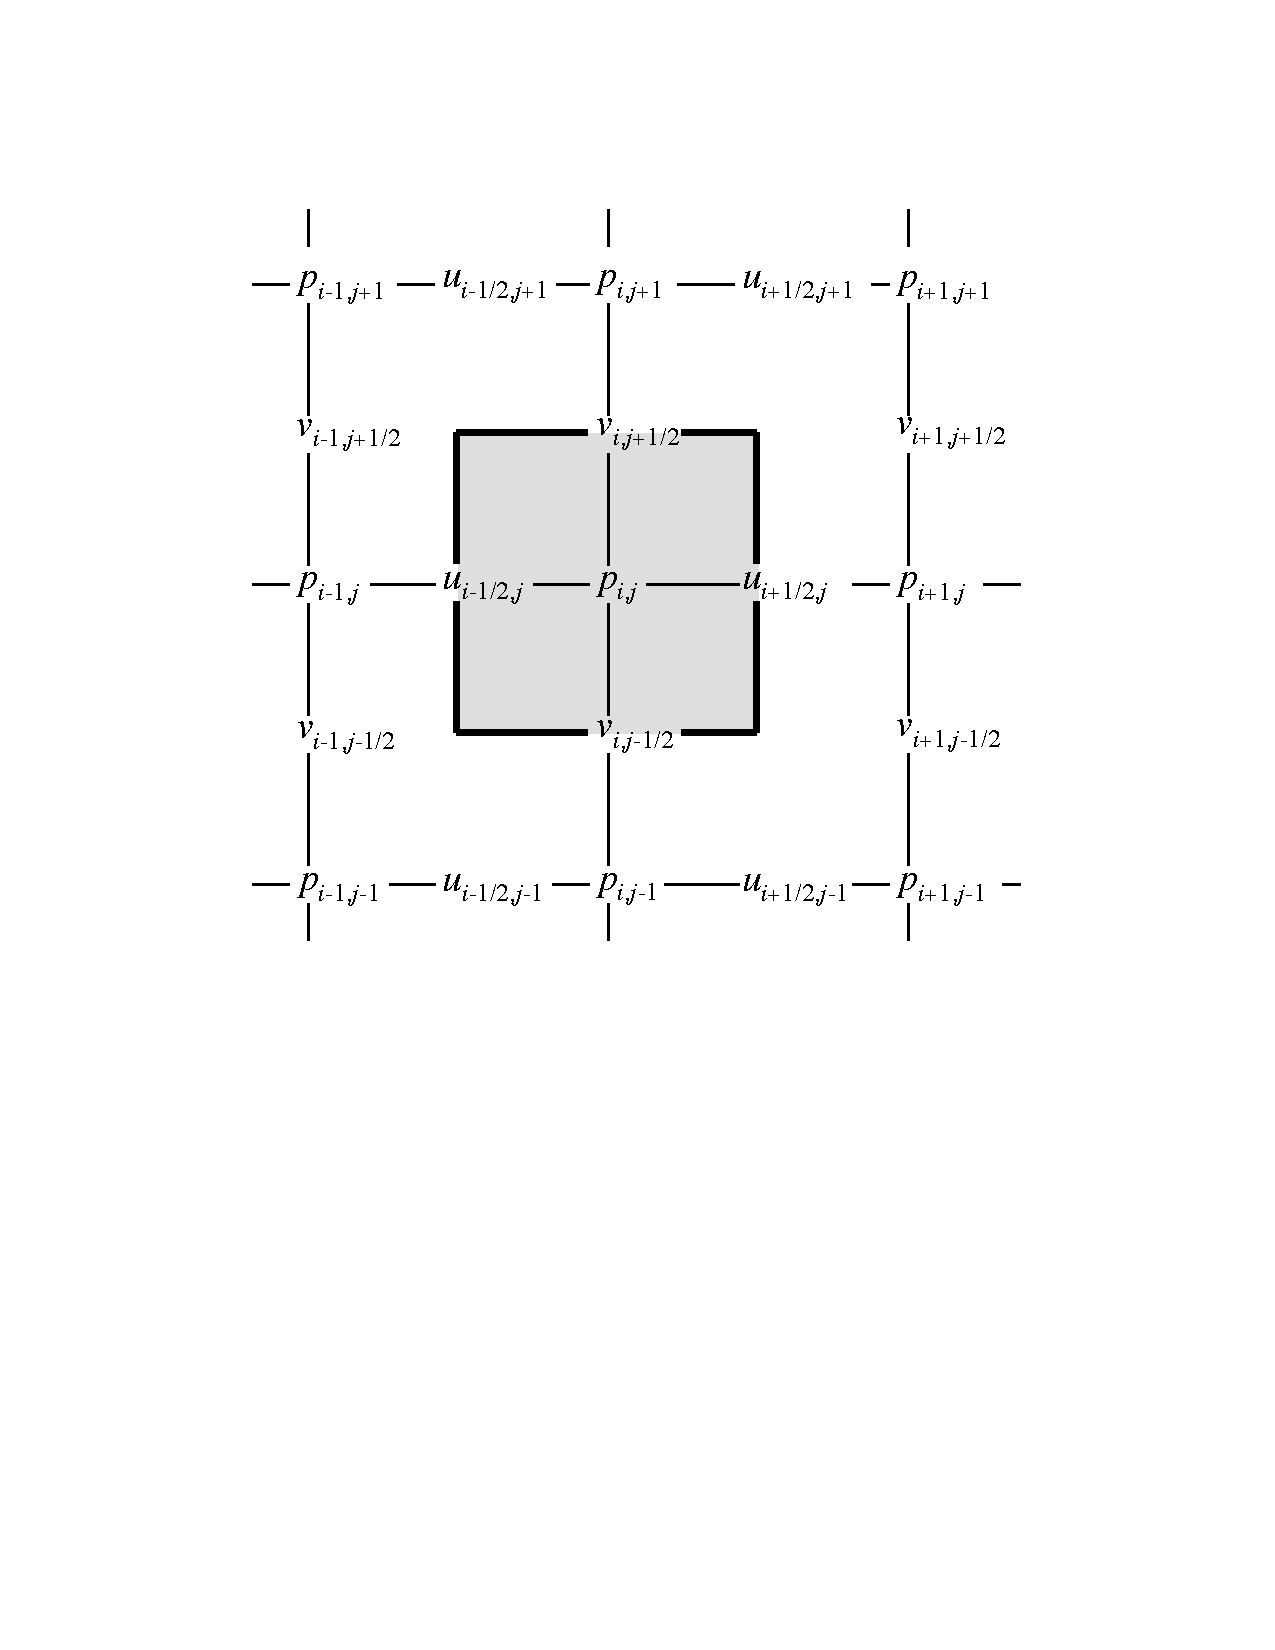
\includegraphics[width=0.45 \textwidth]{Figures/figure3-1.pdf}
\end{center}
\caption{Representation of the staggered spatial discretisation. The pressure $p$ is assumed to 
be known at the center of the control volume outlined by a thick solid line. The horizontal 
velocity component $u_1=u$ is stored in the middle of the left and right edges of this control 
volume and the vertical velocity component $u_2=v$ in the middle of the top and bottom edges.}
\label{stag-grid}
\end{figure}

We assume a regular cubic or square grid. This can be easily
generalized to rectangular or cuboid grids, and with some efforts to
quadtree and octree grids. We also use staggered velocity and pressure
grids. This makes our method more complex than it would be on a
collocated grid. 

The staggered grid is represented in Figure \ref{stag-grid}. In a staggered
grid discretization of the advection equation
the control volumes of the velocity components $u_1$ and $u_2$ are shifted with respect to the
control volume surrounding the pressure $p$.
The use of staggered control volumes has the advantage of
suppressing neutral modes often observed in collocated methods but
leads to more complex discretizations (see \cite{Tryggvason11} for a
more detailed discussion.) The control volumes for $u_1$ and $u_2$ are
shown on Figure \ref{Mac-u-v}. This type of staggered representation
is easily generalized to three dimensions. In what follows we shall
use these control volumes for the velocity or momentum components.

Using the staggered grid leads to a compact expression for the continuity equation
\eqref{divu}
\begin{equation}
{u_{1;i+1/2,j,k}- u_{1;i-1/2,j,k}\over \Delta x}+ 
{u_{2;i,j+1/2,k}- u_{2;i,j-1/2,k}\over \Delta y}+
{u_{3;i,j,k+1/2}- u_{3;i,j,k-1/2}\over \Delta z}=0,
\label{cont2}
\end{equation}
\begin{figure}
\begin{center}{\scalebox{0.4}{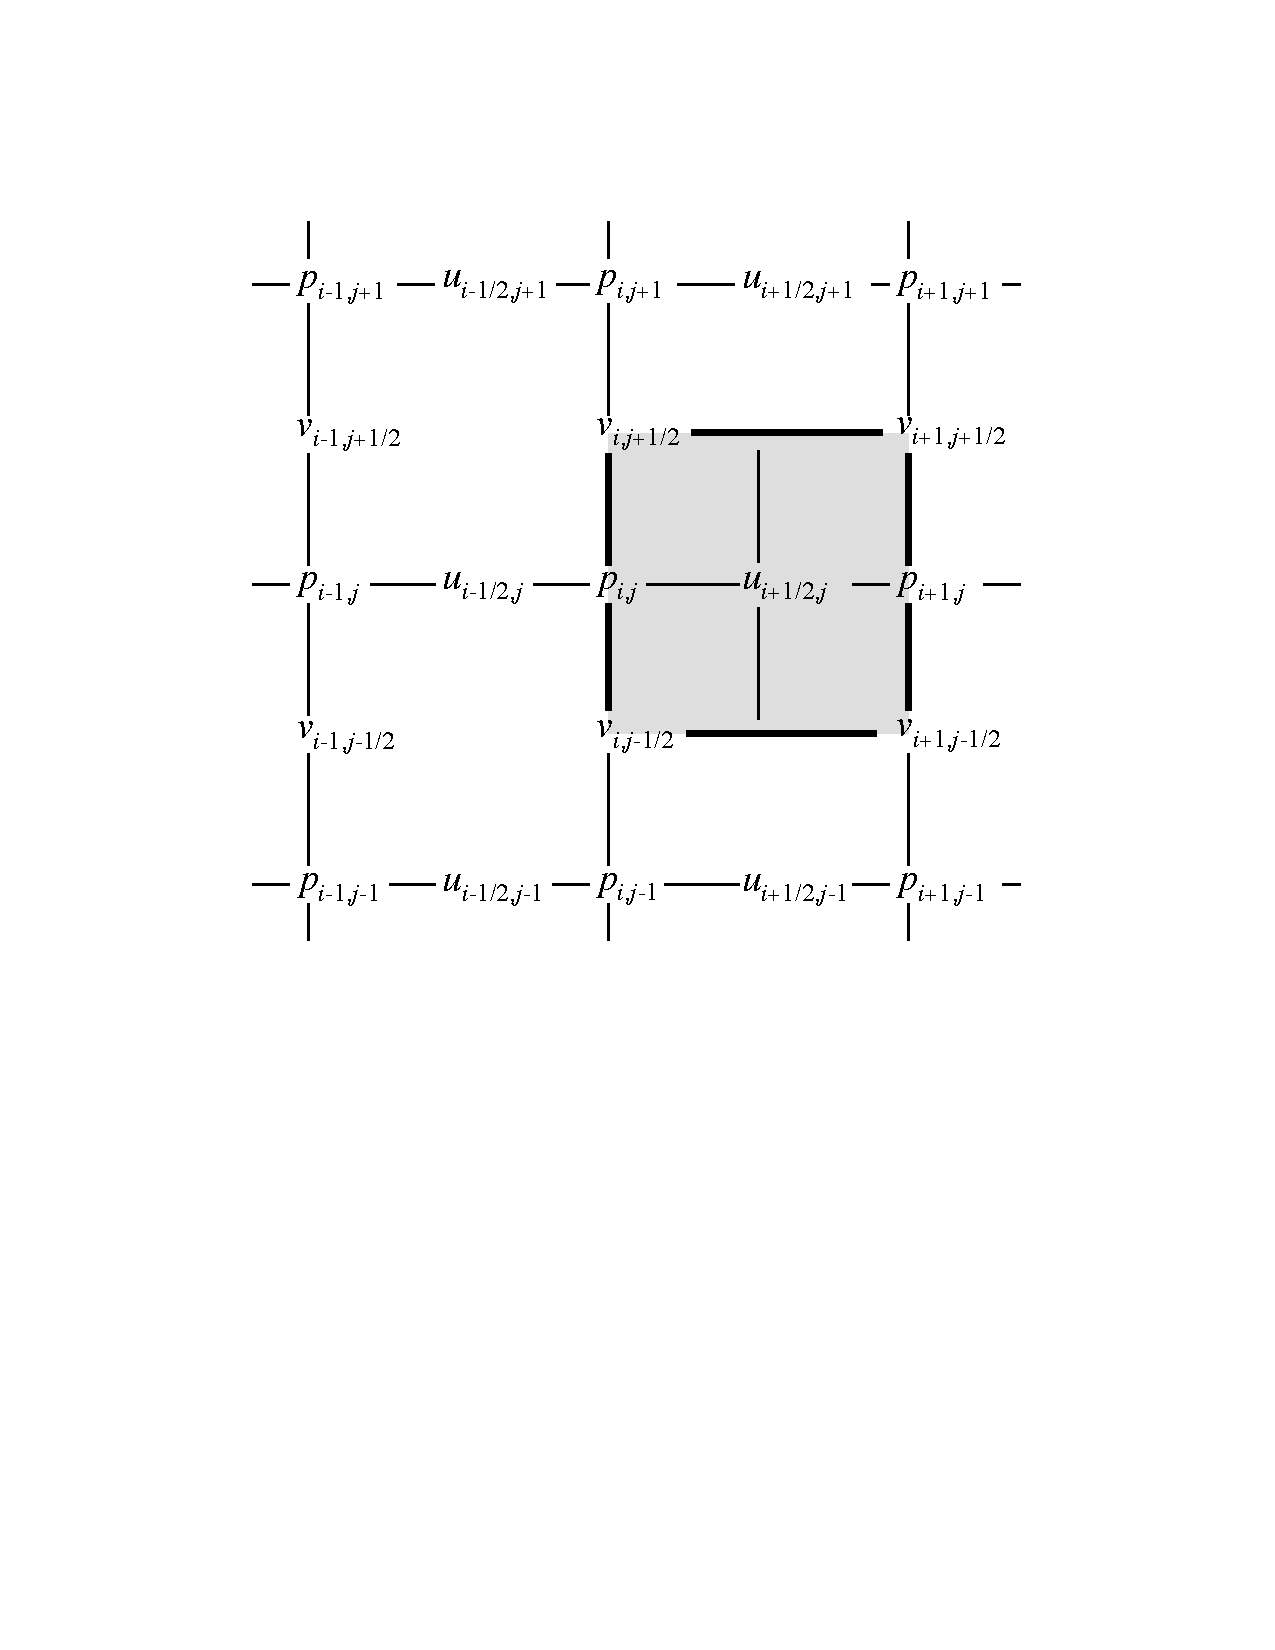
\includegraphics{Figures/figure3-2a.pdf}} \quad
\scalebox{0.4}{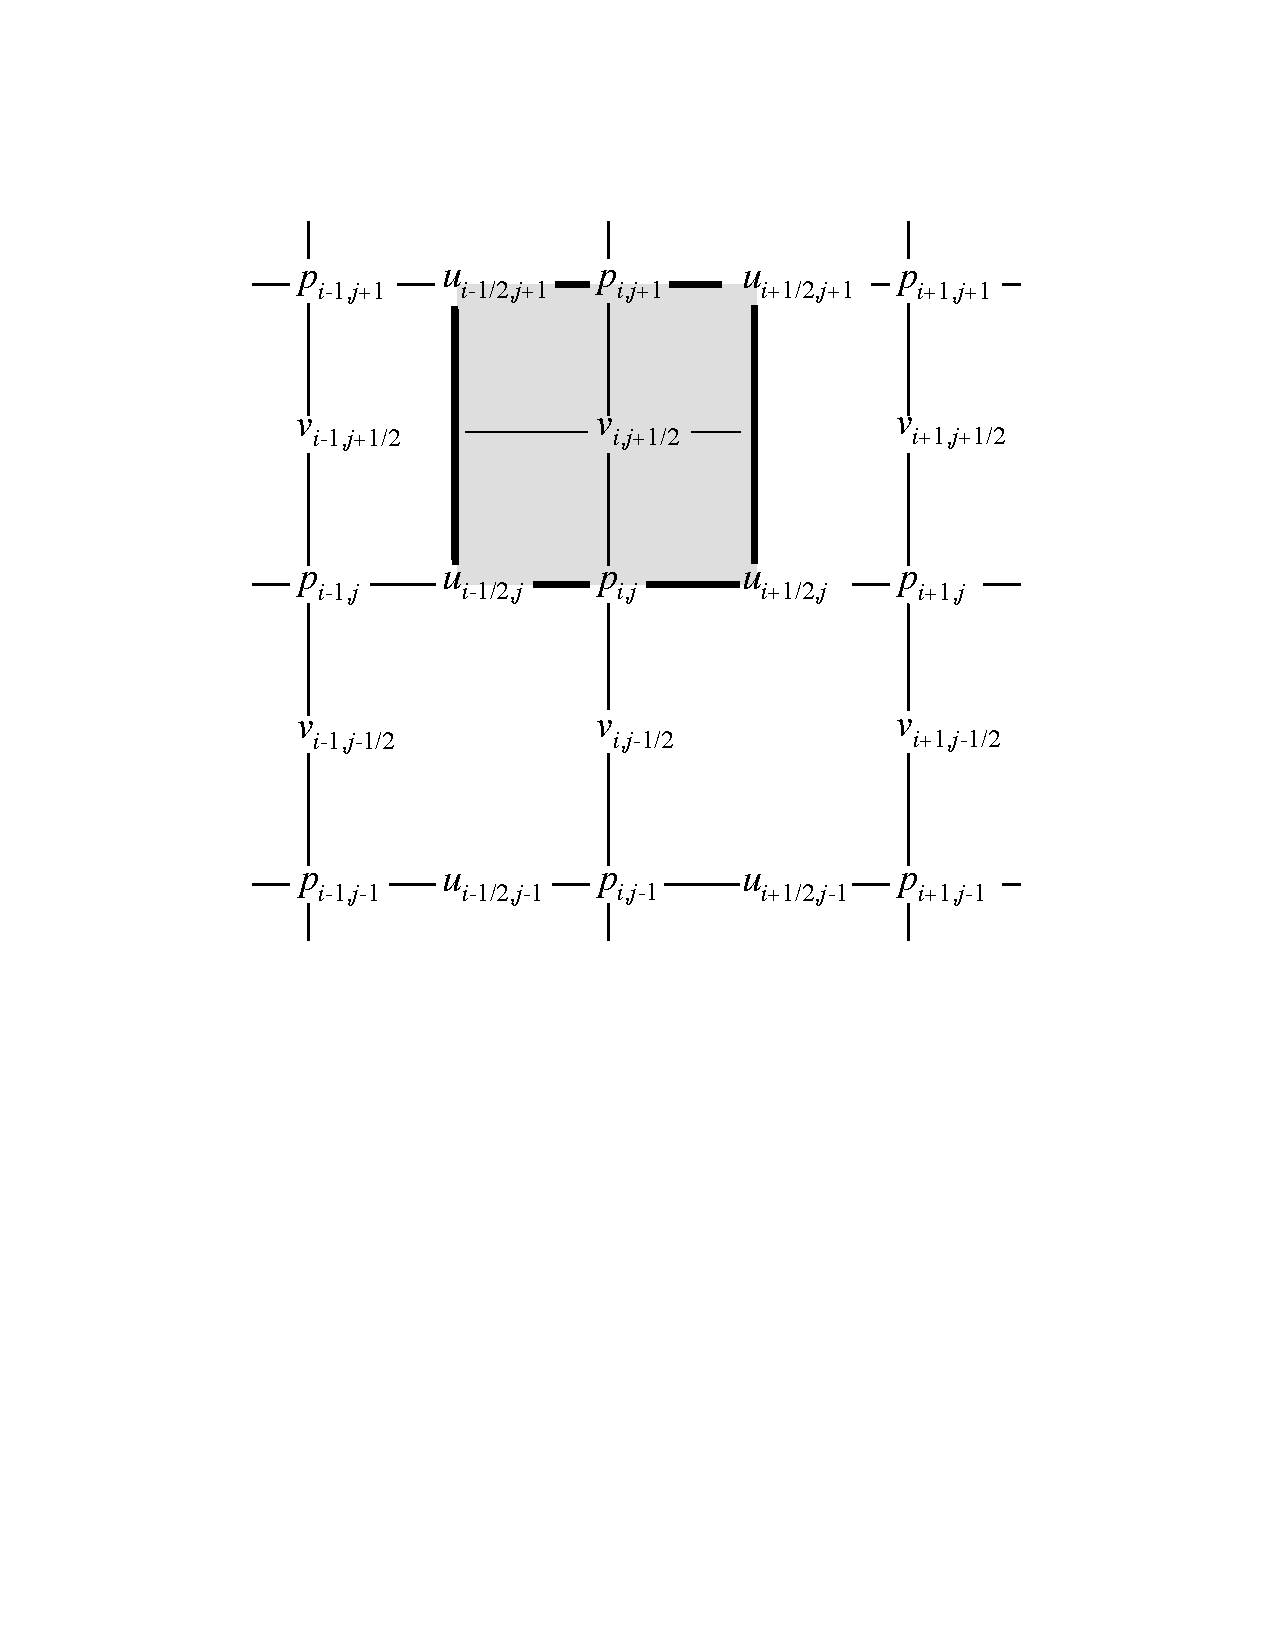
\includegraphics{Figures/figure3-2b.pdf}}  }\\
    (a) \hskip 5cm (b)
\end{center}
\caption{The control volumes for the $u_1=u$ and the $u_2=v$ velocity components are displaced 
half a grid cell to the right (horizontal velocities) and to the top (vertical velocities). Here the 
indices show the location of the stored quantities. Thus, half indices indicate those variables 
stored at the edges of the pressure control volumes.}
\label{Mac-u-v}
\end{figure}
In what follows, we shall use the notation $f=m\pm$, with the integer index $m=1,2,3$,
to note the face of any control volume located in the positive or negative Cartesian direction $m$, 
and $\N_f$ for the normal vector of face $f$ pointing outwards of the control volume.
On a cubic grid the spatial step is
$\Delta x = \Delta y = \Delta z = h$ so the continuity equation becomes
\be
\grad^h \cdot \U = \sum_{m=1}^3 (u_{m+} + u_{m-})/h =0 \,, 
\label{incompdisc3}
\nd
where $u_f=u_{m\pm}= \U \cdot \N_f $ is the velocity normal to face $f$. 
The discretization of the interface location is performed using a VOF method.
VOF methods typically attempt to solve approximately equation (\ref{interfadv}) 
which involves the Heaviside function $H$, whose integral 
in the cell $\Omega$ indexed by $i,j,k$ defines the volume fraction 
$\cijk$ from the relation
\be
h^3 \,\cijk  =\int_\Omega  H  {\rm d}\X \,.
\nd
$\cijk$ represents the fraction of the cell labelled by $i,j,k$ filled with fluid 1, 
taken to be the reference fluid. 
It is worth noting that in the staggered grid setup,
the control volume for $p$ is also the control volume for other scalar quantities,
such as $\rho$ and $H$.

\subsection{Time Marching}

The volume fraction field is updated as
\be
C^{n+1} = C^{n} + \LLL_{\rm VOF}(C^{n},\U^{n}\tau/h) \,,
\label{cnp1}
\nd
where $\LLL_{VOF}$ represents the operator that updates the Volume of Fluid data
given the velocity field. Once volume fraction is updated, the
velocity field is updated in a couple of steps. A projection method is first used, 
in which a provisional velocity field $\U^*$ is computed
\be
\rho^{n+1} \U^* = \rho^n \U^{n} +  \tau \LLL^h_{\rm conv}(\rho^{n},\U^{n}) + \tau \left[\LLL^h_{\rm diff}(\mu^{n},\U^{n}) +  \LLL^h_{\rm cap}(C^{n+1}) + \LLL^h_{\rm ext}(C^{n+1})\right] \label{conspredictedvel}
\nd
It goes without saying that the above operators depend on the discretization steps 
$\tau$ and $h$ as well as the fluid parameters. 
The discussion of the $\LLL^h_{\rm conv}$ operator is the main point of this paper. 
In the second step, the projection step, the pressure gradient force 
is added to yield the velocity at the new time step
\be
\U^{n+1} = \U^* - \frac{\tau }{\rho^{n+1}} \nabla^h p \,. 
\label{fotm}
\nd
The pressure is determined by the requirement that the 
velocity at the end of the time step must be divergence free
\be
\grad^{h} \cdot \ubar^{n+1}=0 \,,
\label{cont-eq1}
\nd
which leads to a Poisson-like equation for the pressure
\be
\grad^h \cdot \frac{\tau }{\rho^{n+1}} \nabla^h p =  \grad^h \cdot \U^* \,.
\nd
